\documentclass[11pt]{article}
\usepackage{fullpage}
\usepackage{authblk}
\usepackage{graphicx}
\usepackage{tikz}
\usepackage{tkz-graph}
\usepackage{amsmath}
\usepackage{amsfonts}
\usepackage{amssymb}
\usepackage{amsthm}
\usepackage{mathrsfs}
\usepackage{enumitem}
\setlist[enumerate]{itemsep=-1mm}
\usepackage{caption}
\usepackage{subcaption}
\captionsetup{compatibility=false} %This is to fix the issue that 'subcaption' package does not work correctly.
%\usepackage[ruled,vlined]{algorithm2e}
\usetikzlibrary{decorations.pathmorphing,arrows}
\usetikzlibrary{decorations.markings}
\tikzset{->-/.style={decoration={markings,mark=at position #1 with {\arrow{>}}},postaction={decorate}}} 

\newtheorem{theorem}{Theorem}%[section]
\newtheorem{lemma}[theorem]{Lemma}
\newtheorem{claim}[theorem]{Claim}
\newtheorem{corollary}[theorem]{Corollary}
\newtheorem{proposition}[theorem]{Proposition}
\newtheorem{definition}[theorem]{Definition}
\newtheorem{remark}[theorem]{Remark}
\newtheorem{assumption}[theorem]{Assumption}
\newtheorem{hypothesis}[theorem]{Hypothesis}
\newtheorem{observation}[theorem]{Observation}

\numberwithin{theorem}{section}

\makeatletter
\renewcommand\section{%
  \@startsection{section}{1}
                {\z@}%
                {-3.5ex \@plus -1ex \@minus -.2ex}%
                {2.3ex \@plus.2ex}%
                {\large\bfseries}% 11pt
}
\renewcommand\subsection{%
  \@startsection{subsection}{2}
                {\z@}%
                {-3.25ex\@plus -1ex \@minus -.2ex}%
                {1sp}% No space after subsections
                {\normalsize\bfseries}% normal size, boldface
}
\renewcommand\subsubsection{%
  \@startsection{subsubsection}{3}
                {\z@}%
                {-3.25ex\@plus -1ex \@minus -.2ex}%
                {1sp}% No space after subsubsections
                {\normalfont\normalsize}% normal size, medium
}
\makeatother

\marginparwidth 0pt \oddsidemargin 0pt \evensidemargin 0pt
\topmargin 30pt \textheight 21.0 truecm \textwidth 16.0 truecm

\title{{\Large\bf  Strongly Kernel Mengerian Orientations of Line Multigraphs}}


\author{}

\begin{document}

\date{\today}

\numberwithin{equation}{section}

\maketitle
%\thispagestyle{empty}

\openup 1.2\jot

\begin{abstract}
Given an digraph $D$, $\sigma(D)$ denotes the linear system consisting of domination, independence and nonnegativity constraints, and $FK(D)$ denotes the set of all solutions of $\sigma(D)$. We call $D$ is strongly kernel ideal if $FK(D')$ is integral for each induced subgraph $D'$ of $D$ and strongly kernel Mengerian if $\sigma(D')$ is TDI for each induced subgraph $D'$ of $D$. Given a preference system $(G,\prec)$, $\pi(G,\prec)$ denotes the Rothblum system for $(G,\prec)$ and $FSM(G,\prec)$ denotes all solution of $\pi(G,\prec)$. 

In this paper, we prove that  $D$ is a `good' orientation of line multigraph $L(H)$ iff $D$ is kernel ideal iff $D$ is kernel Mengerian. We construct a preference system $(H,\prec)$ from each `good' orientation $D$ such that $FK(D)=FSM(H,\prec)$. Then we work on a projection $FSM(\hat{H},\hat\prec)$ of $FSM(H,\prec)$ where $(\hat{H},\hat\prec)$ is a preference subsystem of $(H,\prec)$ such that $\hat{H}$ is a underlying simple graph of $H$ and $\hat\prec$ is the restriction of $\prec$ onto $\hat{H}$. We prove our results by showing that $FK(D)$ is integral iff $FSM(\hat{H},\hat\prec)$ is integral and $\sigma(D)$ is TDI if $\pi(\hat{H},\hat\prec)$ is TDI.
\end{abstract}

\section{Introduction}
\label{intro}
Let $G$ be a undirected graph. We call $G$ \textit{simple} if it contains no loops or parallel edges and call $G$ a \textit{multigraph} if it contains no loops but parallel edges are allowed. 

The \textit{line graph} of a undirected graph $G$ is a undirected simple graph that represents the adjacency of edges of $G$. The \textit{line multigraph} of a undirected graph $G$ is a undirected multigraph that represents the adjacencies of edges of $G$ and if edges $e$ and $f$ have two common ends in $G$, their corresponding vertices are joined by two edges. In this paper, line graphs and line multigraphs of $G$ are both denoted by $L(G)$ if no ambiguity occurs. Observe that the line graph and line multigraph of $G$ are the same when $G$ is simple. And for any two vertices in a line multigraph, they have at most two parallel edges between them.

A \textit{digraph} is a graph, where edges have a direction associated with them. \textit{Simple} digraphs and \textit{multidigraphs} are defined analogously to simple graphs and multigraphs. An \textit{orientation} of a undirected graph $G$ is a digraph obtained by orienting each edge of $G$ in either direction. A \textit{clique} of $G$ (\textit{resp.} $D$) is a subset of vertex set of $G$ (\textit{resp.} $D$) such that every two distinct vertices are adjacent. An orientation of $G$ is \textit{clique-acyclic} if for every clique of $G$ the induced subdigraph of one-way arcs is acyclic. 
 
Let $D=(V,A)$ be a digraph. We call $U\subseteq V$ an \textit{independent} set of $D$ if no two vertices in $U$ are connected by an arc, call $U$ a \textit{dominating} set of $D$ if for each vertex $v\not\in U$, there is an arc from $v$ to $U$, and call $U$ a \textit{kernel} of $D$ if it is both independent and dominating. 
We call $D$ \textit{good} if it is clique-acyclic and each directed odd cycle has a chord or a pseudochord\footnote{A pseudochord is an arc $(v_i,v_{i-1})$ in a directed cycle $v_1 v_2\ldots v_l$}. 

\begin{theorem}[Borodin \textit{et al.} \cite{BoroKost98}]
\label{thm:BoroKost98}
Let $G$ be a line multigraph. The orientation $D$ of $G$ is kernel perfect if and only if it is good.
\end{theorem}

A subset $P$ of $\mathbb{R}^n$ is called a \textit{polytope} if it is the convex hull of finitely many vectors in $\mathbb{R}^n$. A point $x$ in $P$ is called a \textit{vertex} or an \textit{extreme point} if there exist no distinct points $y$ and $z$ in $P$ such that $x=\alpha y+ (1-\alpha)z$ for $0<\alpha<1$. It is well known that $P$ is the convex hull of its vertices, and that there exists a linear system $Ax\leq b$ such that $P=\{x\in\mathbb{R}^n:Ax\leq b\}$. We call $P$ $1/k$-\textit{integral} if its vertices are $1/k$-integral vectors, where $k\in\mathbb{N}$. By a theorem in linear programming, $P$ is $1/k$-integral if and only if $\max\{c^T x:Ax\leq b\}$ has an optimal $1/k$-integral solution, for every integral vector $c$ for which the optimum is finite. If, instead, $\max\{c^T x:Ax\leq b\}$ has a dual optimal $1/k$-integral solution, we call linear system $Ax\leq b$ \textit{totally dual $1/k$-integral} (TDI$/k$).
It is easy to verify that $Ax\leq b$ is TDI$/k$ if and only if $Bx\leq b$ is TDI, where $B=A/k$. Thus, from a theorem by Edmonds and Giles \cite{EdmoGile77}, we deduce that if $Ax\leq b$ is TDI$/k$ and $b$ is integal, then $P=\{x\in\mathbb{R}^n:Ax\leq b\}$ is $1/k$-integral.

Let $\sigma(D)$ denote the linear system consisting of the following inequalities:
\begin{alignat}{4}
x(v)+x(N^+_{D}(v)) &\geq 1 &\qquad &\forall ~ v~&\in V, \label{domination constraints}\\
x(Q)&\leq 1 &\qquad &\forall ~ Q &\in \mathcal{Q}, \label{independence constraints}\\
x(v) &\geq 0 &\qquad &\forall ~ v~&\in V, \label{vertex nonnegativity}
\end{alignat}
where $x(U)=\sum_{u\in U}x(u)$ for any $U\subseteq V$, $N_D^+(v)$ denotes the set of all out-neighbors of vertex $v$, and $\mathcal{Q}$ denotes the collection of all cliques of $D$. Observe that incidence vectors of kernels of $D$ are precisely integral solutions $x\in \mathbb{Z}^A$ of $\sigma(D)$.

The \textit{kernel polyotpe} of $D$, denoted by $K(D)$, is the convex hull of incidence vectors of all kernels of $D$.  The \textit{fractional kernel polytope} of $D$, denoted by $FK(D)$, is the set of all solutions $x\in \mathbb{R}^A$ of $\sigma(D)$. Clearly, $K(D)\subseteq FK(D)$.

We call $D$ \textit{kernel perfect} if each of its induced subgraphs has a kernel, \textit{strongly kernel ideal} if $FK(D')$ is integral for each induced subgraph $D'$ of $D$, and \textit{strongly kernel Mengerian} if $\sigma(D')$ is TDI for each induced subgraph $D'$ of $D$.

According to EGRES open, the polyhedral description of kernels remains open. One attempt on a polyhedral description of kernels is made by Chen \textit{et al.} \cite{ChenChen16} where they replace clique constraints $x(Q)\leq 1$ for $Q\in\mathcal{Q}$ with independence constraints $x(u)+x(v)\leq 1$ for $(u,v)\in A$. In this paper we show that the polyhedral description of kernels in orientations of line multigraphs can be thoroughly characterized by reducing the problem to a stable matching problem.

\begin{theorem}
\label{thm:main}
Let $G$ be a line multigraph, and let $D$ be an orientation of $G$. Then the following statements are equivalent:
\begin{enumerate}[label={\emph{(}\roman*\emph{)}}]
	\item $D$ is good;
	\item $D$ is kernel perfect;
	\item $D$ is strongly kernel ideal;
	\item $D$ is strongly kernel Mengerian.
\end{enumerate}
\end{theorem}

The equivalence of $(i)$ and $(ii)$ was established by Theorem \ref{thm:BoroKost98} (see Maffray \cite{Maff92} for the case when $G$ is perfect line graphs). Kir\'{a}ly and Pap \cite{KiraPap08} proved the theorem for the case when $G$ is the line graph of a bipartite graph.	 Our paper generalizes the result of Kir\'{a}ly and Pap to general line multigraphs.


\section{Preliminaries}
\label{pre}
Let $G=(V,E)$ be a undirected graph. For each $v\in V$, let $\delta(v)$ be the set of all edges incident to $v$ and let $\prec_v$ be a strict linear order on $\delta(v)$. We call $\prec_v$ the \emph{preference} of $v$ and say that $v$ \emph{prefers} $e$ to $f$ if $e\prec_v f$. Let $\prec$ be collection of all these $\prec_v$ for $v\in V$. We call the pair $(G,\prec)$ a \emph{preference system}. An edge $e$ is said to dominate another edge $f$ if they have a common end $v$ such that $e\preceq_v f$. Let $M$ be a matching of $G$. We call $M$ \emph{stable} if each edge of $G$ is dominated by some edge in $M$.

Let $(G,\prec)$ be a preference system. For each $e\in E$, let $\varphi(e)$ denote the set of all edges of $G$ that dominate $e$. Let $\pi(G,\prec)$ be the linear system consisting of the following inequalites:
\begin{alignat}{3}
x(\varphi(e)) &\geq 1 &\qquad \forall ~e &\in E,\label{stability constraints}\\
x(\delta(v)) &\leq 1 &\qquad \forall ~v &\in V,\label{matching constraints}\\
x(e) &\geq 0 &\qquad \forall ~e &\in E.\label{edge nonnegativity}
\end{alignat}
As observed by Abeledo and Rothblum, incidence vectors of stable matchings of $(G,\prec)$ are precisely integral solutions $x\in \mathbb{Z}^E$ of $\pi(G,\prec)$.

The \textit{stable matching polytope}, denoted by $SM(G,\prec)$, is the convex hull of incidence vectors of all stable matchings of $(G,\prec)$. The \textit{fractional stable matching polytope}, denoted by $FSM(G,\prec)$, is the set of all solutions $x\in \mathbb{R}^E$ of $\pi(G,\prec)$. Clearly, $SM(G,\prec)\subseteq FSM(G,\prec)$. 

\begin{theorem}[Rothblum \cite{Roth92}]
\label{thm:Roth92}
Let $(G,\prec)$ be a preference system. If $G$ is bipartite, then
$SM(G,\prec)=FSM(G,\prec)$.
\end{theorem}

\begin{theorem}[Kir\'{a}li and Pap \cite{KiraPap08}]
\label{thm:KiraPap08}
Let $(G,\prec)$ be a preference system. If $G$ is bipartite, then $\pi(G,\prec)$ is totally dual integral.
\end{theorem}

Let $C=v_1 v_2 \ldots v_l$ be a cycle in $G$, we say that $C$ has \textit{cyclic preferences} in $(G,\prec)$ if
$v_{i-1} v_i \prec_{v_i} v_i v_{i+1}$ for $i=1,2,\ldots,l$
or $v_{i-1} v_i\succ_{v_i} v_i v_{i+1}$ for $i=1,2,\ldots,l$,
where $i+1$ is taken modulo $l$.
For $x\in FSM(G,\prec)$, $E_{\alpha}(x)$ denotes the set of all edges with $x(e)=\alpha$ for $\alpha\in\mathbb{R}$.

\begin{theorem}[Abeledo and Rothblum \cite{AbelRoth94}]
\label{thm:AbelRoth94}
Let $(G,\prec)$ be a preference system. Then $FSM(G,\prec)$ is $1/2$-integral. Moreover, for every $1/2$-integral point $x$ in $FSM(G,\prec)$, $E_{1/2}(x)$ consists of vertex disjoint cycles with cyclic preferences.
\end{theorem} 

\begin{theorem}[Chen \textit{et al.} \cite{ChenDing12}]
\label{thm:ChenDing12}
Let $(G,\prec)$ be a preference system. Then $\pi(G,\prec)$ is totally dual $1/2$-integral. Moreover, $\pi(G,\prec)$ is totally dual integral if and only if $SM(G,\prec)=FSM(G,\prec)$.
\end{theorem}

\section{Reductions}
Observe that to study kernels in multidigraphs, it suffices to work on its minimal spanning subdigraph that  preserves all the connection relations among vertices. Hence in the reaming of this paper, we assume that $D$ is a multidigraph such that any two vertices are joined by at most one arc in each direction. For simplicity, we further assume that $D$ is an orientation of a line multigraph $L(H)$ such that any two vertices in $H$ are joined by at most two edges and parallel edges in $L(H)$ are orientated oppositely.

Kernels are closely related to stable matchings. Kernels in a clique-acyclic orientation $D$ of a line multigraph $L(H)$ correspond to stable matchings in the preference system $(H,\prec)$, where preferences $\prec$ are uniquely determined by orientations: for any two adjacent edges $e$ and $f$ in $H$, we define $e\prec_v f$ if $(e,f)$ is an arc in $D$. 
Hence each clique-acyclic orientation $D$ of a line multigraph $L(H)$ is associated with a preference system $(H,\prec)$.

In the remaining of this paper, we always assume that $D$ is a clique-acyclic orientation of a line multigraph $L(H)$ and use $(H,\prec)$ to denote the preference system constructed from $D$. Recall that $\sigma(D)$ denotes the linear system which defines $FK(D)$. Consequently, $\sigma(D)$ has an interpretation in terms of preference system $(H,\prec)$. The equivalence of constraints (\ref{vertex nonnegativity}) and constraints (\ref{edge nonnegativity}) follows directly. Constraints (\ref{domination constraints}) can be viewed as constraints (\ref{stability constraints}) because of the one to one correspondence between dominating vertex set $\{v\}\cup N^+_D(v)$ for $v\in V(D)$ and stable edge set $\varphi(e)$ for $e\in E(H)$.
Observe that cliques of $D$ correspond to three types of edge sets in $H$:
\begin{itemize}
\item $\delta(v)$ for $v\in V(H)$,
\item nontrivial subsets of $\delta(v)$ for $v\in V(H)$,
\item 3-cycles in $H$.
\end{itemize}
Hence constraints (\ref{independence constraints}) can be viewed as constraints (\ref{matching constraints}) together with some extra constraints on $(H,\prec)$. Let $\mathcal{O}(H)$ denote the collection of all $3$-cycles in $H$. It follows that $\sigma(D)$ can be viewed as a linear system defined on preference system $(H,\prec)$:
\begin{alignat}{4}
x(\varphi(e)) &\geq 1 &\qquad &\forall ~e &\in E(H),\label{constraints:1}\\
x(\delta(v)) &\leq 1 &\qquad &\forall ~v &\in V(H),\label{constraints:2}\\
x(S) &\leq 1 &\qquad \emptyset\subset S\subset \delta(v),\quad &\forall ~v&\in V(H),\label{constraints:3}\\
x(O) &\leq 1 &\qquad &\forall ~O&\in \mathcal{O}(H),\label{constraints:4}\\
x(e) &\geq 0 &\qquad &\forall ~e &\in E(H)\label{constraints:5}.
\end{alignat}

Notice that constraints (\ref{constraints:1}), (\ref{constraints:2}) and (\ref{constraints:5}) form the Rothblum system $\pi(H,\prec)$ which defines $FSM(H,\prec)$. Constraints (\ref{constraints:3}) are redundant for defining $FK(D)$ due to constraints (\ref{constraints:2}). It turns out that constraints (\ref{constraints:4}) are also redundant for defining $FK(D)$ when $D$ is good. Therefore, $FK(D)$ is essentially defined by Rothblum system $\pi(H,\prec)$, or equivalently $FK(D)=FSM(H,\prec)$, when $D$ is good.

Notice that $H$ in preference system $(H,\prec)$ is a multigraph. We have the following observation for parallel edges in preference system $(H,\prec)$.

\begin{lemma}
\label{lem:reduct1}
For parallel edges $e$ and $e'$ in $E(H)$, there exists no edge $f$ such that $e\prec_v f \prec_v e'$ or $e'\prec_u f\prec_u e$, where $u$ and $v$ are endpoints of $e$ and $e'$.
\end{lemma}
\begin{proof}
Since $D$ is clique-acyclic, the lemma follows directly.
\end{proof}

By Lemma \ref{lem:reduct1}, parallel edges play the same role in preference system $(H,\prec)$. Hence it suffices to work on preference systems defined on its underlying simple graphs. We use $(\hat{H},\hat\prec)$ to denote the preference subsystem of $(H,\prec)$, where $\hat{H}$ is a spanning subgraph of $H$ obtained by keeping one edge between every pair of adjacent vertices in $H$ and $\hat\prec$ is the restriction of $\prec$ on $\hat{H}$. Before we proceed, we introduce a technical lemma first.

\begin{lemma}
\label{lem:reduct2}
Let 
\begin{equation}\label{equ:syst.}
Ax\leq b,~x\geq 0
\end{equation}
and
\begin{equation}\label{equ:syst. with duplicate columns}
\bar{A}\bar{x}\leq b,~\bar{x}\geq 0
\end{equation}
be two linear systems, where $\bar{A}$ is obtained from $A$ by duplicating some columns. If (\ref{equ:syst.}) is totally dual $1/k$-integral, then so is (\ref{equ:syst. with duplicate columns}), where $k\in \mathbb{N}$.
\end{lemma}
\begin{proof}
It suffices to prove that the theorem holds for $\bar{A}$ with one duplicate column.
Let $\bar{x}=(\bar{x}_1,\ldots,\bar{x}_{n+1})\in\mathbb{R}^{n+1}$ and $\bar{A}=(\bar{a}_1,\ldots,\bar{a}_{n+1})=(A,a_{k})$, where $a_k$ is the $k$th column of $A$. Let $\bar{c}=(\bar{c}_1,\ldots,\bar{c}_{n+1})\in \mathbb{Z}^{n+1}$ be an arbitrary integral vector such that $\max\{\bar{c}^T \bar{x}: \bar{A}\bar{x}\leq b,~\bar{x}\geq 0\}$ is finite. 

Let $\hat{c}\in \mathbb{Z}^n$ be defined by
\begin{equation*}
\hat{c}_i=
\begin{cases}
\bar{c}_i & i\not=k,\\
\max\{\bar{c}_k, \bar{c}_{n+1}\} & i=k,
\end{cases}
\end{equation*}
and $\hat{x}\in \mathbb{R}^n$ be defined by
\begin{equation*}
\hat{x}_i=
\begin{cases}
\bar{x}_i & i\not=k,\\
\bar{x}_k+\bar{x}_{n+1} & i=k.
\end{cases}
\end{equation*}
Clearly,  $\max\{\hat{c}^T \hat{x}:A\hat{x}\leq b,~\hat{x}\geq 0\}\geq\max\{\bar{c}^T \bar{x}:\bar{A}\bar{x}\leq b,~\bar{x}\geq 0\}$. We claim that equality always holds in this inequality. Given an arbitrary optimal solution $\hat{x}^*$ to $\max\{\hat{c}^T \hat{x}:A\hat{x}\leq b,~\hat{x}\geq 0\}$, define $\bar{x}^*$ by $\bar{x}^*_i=\hat{x}^*_i$ for $i\not=k,n+1$, if $\bar{c}_k>\bar{c}_{n+1}$, $\bar{x}^*_k=\hat{x}^*_k$ and $\bar{x}^*_{n+1}=0$, otherwise $\bar{x}^*_k=0$ and $\bar{x}^*_{n+1}=\hat{x}^*_k$. It is easy to verify that $\bar{x}^*$ is a feasible solution to $\max\{\bar{c}^T \bar{x}:\bar{A}\bar{x}\leq b,~\bar{x}\geq 0\}$. Moreover, $\hat{c}^T\hat{x}^*=\bar{c}^T\bar{x}^*$ implies $\max\{\hat{c}^T \hat{x}:A\hat{x}\leq b,~\hat{x}\geq 0\}\leq\max\{\bar{c}^T \bar{x}:\bar{A}\bar{x}\leq b,~\bar{x}\geq 0\}$. Hence equality follows.

Since $Ax\leq b$ is TDI$/k$, there exists a dual optimal $1/k$-integral solution $y^*$ to $\max\{\hat{c}^T\hat{x}:A\hat{x}\leq b,~\hat{x}\geq 0\}$ such that $(y^*)^T b=\max\{\hat{c}^T \hat{x}:A\hat{x}\leq b,~\hat{x}\geq 0\}$, $(y^*)^T A\geq \hat{c}^T$ and $y^*\geq 0$. It follows that
\begin{equation*}
(y^*)^T \bar{A}=(y^*)^T (A,a_k)=((y^*)^T A,(y^*)^T a_k)\geq (\hat{c}^T,\hat{c}_k)\geq\bar{c}^T,
\end{equation*}
implying that $y^*$ is a feasible dual solution to $\max\{\bar{c}^T \bar{x}:\bar{A}\bar{x}\leq b,~\bar{x}\geq 0\}$. By the following inequalities
\begin{equation*}
(y^*)^T b=\max\{\hat{c}^T \hat{x}:A\hat{x}\leq b,~\hat{x}\geq 0\}=\max\{\bar{c}^T \bar{x}:\bar{A}\bar{x}\leq b,~\bar{x}\geq 0\}\leq (y^*)^T b,
\end{equation*} $y^*$ is also a dual optimal solution to $\max\{\bar{c}^T \bar{x}:\bar{A}\bar{x}\leq b,~\bar{x}\geq 0\}$, where the last inequality is from the weak duality theorem. Hence the lemma follows.
\end{proof}

\begin{lemma}
\label{lem:reduct3}
If $\pi(\hat{H},\hat\prec)$ is totally dual $1/k$-integral, then so is $\pi(H,\prec)$, where $k\in\mathbb{N}$.
\end{lemma}
\begin{proof}
By Lemma \ref{lem:reduct1}, columns in the left hand side matrix of $\pi(H,\prec)$ corresponding to parallel edges are identical. Hence the left hand side matrix of $\pi(H,\prec)$ can be obtained from that of $\pi(\hat{H},\hat\prec)$ by duplicating columns corresponding to parallels edges. Then the lemma follows from Lemma \ref{lem:reduct2}.
\end{proof}

\begin{lemma}
\label{lem:reduct4}
$FSM(H,\prec)$ is $1/2$-integral. Moreover, for each vertex $x$ of $FSM(H,\prec)$, there exists no parallel edges $e$ and $e'$ such that $x(e)=x(e')=1/2$.
\end{lemma}
\begin{proof}
By Theorem \ref{thm:ChenDing12}, $\pi(\hat{H},\hat\prec)$ is TDI$/2$. Hence $\pi(H,\prec)$ is also TDI$/2$ by Lemma \ref{lem:reduct3}. From a theorem by Edmonds and Giles \cite{EdmoGile77}, it follows that $FSM(H,\prec)$ is $1/2$-integral.

To see the second part of this lemma, consider an arbitrary vertex $x$ of $FSM(H,\prec)$. Notice that whenever $x(e)=x(e')=1/2$ for parallel edges $e$ and $e'$, we have $x=1/2 (x_1 + x_2)$ where $x_1$ is obtained from $x$ by setting $x_1 (e)=1$ and $x_1 (e')=0$ and $x_2$ is obtained from $x$ by setting $x_1 (e)=0$ and $x_1 (e')=1$. Clearly, $x_1, x_2\in FSM(H,\prec)$, contradicting to the fact that $x$ is a vertex.
\end{proof}

\begin{lemma}
\label{lem:reduct5}
$FSM(\hat{H},\hat\prec)$ is a projection of $FSM(H,\prec)$. Moreover, each vertex of $FSM(H,\prec)$ can be obtained from some vertex of $FSM(\hat{H},\hat\prec)$ by adding some zero entries. 
\end{lemma}
\begin{proof}
For simplicity, let $H=(V,E)$ and $\hat{H}=(V,\hat{E})$.
For an arbitrary point $\hat{x}\in FSM(\hat{H},\hat\prec)$, define $x=(\hat{x},0)\in \mathbb{R}^{\hat{E}}\times \mathbb{R}^{E-\hat{E}}$. To show that $x\in FSM(H,\prec)$, it suffices to prove that $x(\varphi(e))\geq 1$ for $e\in E-\hat{E}$. Let $e'\in \hat{E}$ be the edge parallel with $e\in E-\hat{E}$. By Lemma \ref{lem:reduct1}, $x(\varphi(e))=x(\varphi(e'))=\hat{x}(\varphi(e'))\geq 1$. Hence $FSM(\hat{H},\hat\prec)$ is a projection of $FSM(H,\prec)$

Let $x$ be a vertex of $FSM(H,\prec)$. Define $\hat{x}\in \mathbb{R}^{\hat{E}}$ by, for $e\in \hat{E}$, $\hat{x}(e)=x(e)+x(e')$, where $e'\in E-\hat{E}$ is parallel with $e$. By Lemma \ref{lem:reduct1}, it is easy to verify that $\hat{x}\in FSM(\hat{H},\hat\prec)$. We claim that $\hat{x}$ is a vertex of $FSM(\hat{H},\hat\prec)$. Assume to the contrary that there exist $\hat{x}_1, \hat{x}_2 \in FSM(\hat{H},\hat\prec)$ such that $\hat{x}=\alpha \hat{x}_1+ (1-\alpha)\hat{x}_2$, for $0<\alpha<1$. For $i=1,2$, we extend $\hat{x}_i\in \mathbb{R}^{\hat{E}}$ to $x_i\in \mathbb{R}^{E}$ by, for $e\in \hat{E}$ without parallel edges in $H$, $x_i(e)=\hat{x}_i(e)$; for $e\in\hat{E}$ and its parallel edge $e'\in E-\hat{E}$, if $x(e)>x(e')$, $x_i(e)=\hat{x}_i(e)$ and $x_i(e')=0$, otherwise $x_i(e)=0$ and $x_i(e')=\hat{x}_i(e)$. By Lemma \ref{lem:reduct1}, it is easy to see that $x_1,x_2\in FSM(H,\prec)$. And by Lemma \ref{lem:reduct4}, $x(e)\cdot x(e')=0$ for every pair of parallel edges $e$ and $e'$. Hence $x=\alpha x_1+(1-\alpha) x_2$ follows, contradicting to the assumption that $x$ is a vertex. Therefore, $\hat{x}$ is vertex of $FSM(\hat{H},\hat\prec)$. It follows that each vertex $x$ of $FSM(H,\prec)$ is associated with a vertex $\hat{x}$ of $FSM(\hat{H},\hat\prec)$ and $x$ can be obtained from $\hat{x}$ by, for $e\in \hat{E}$ without parallel edges in $H$, $x(e)=\hat{x}(e)$; for $e\in\hat{E}$ and its parallel edge $e'\in E-\hat{E}$, if $x(e)>x(e')$, $x(e)=\hat{x}(e)$ and $x(e')=0$, otherwise $x(e)=0$ and $x(e')=\hat{x}(e)$. 
\end{proof}

\begin{lemma}
\label{lem:reduct6}
$FSM(H,\prec)$ is integral if and only if $FSM(\hat{H},\hat\prec)$ is integral.
\end{lemma}
\begin{proof}
The only if part is well known since by the first part of Lemma \ref{lem:reduct5}, $FSM(\hat{H},\hat\prec)$ is a projection of $FSM(H,\prec)$. The if part follows directly from the second part of Lemma \ref{lem:reduct5}.
\end{proof}


\section{Proofs}
As observed by Borodin \textit{et al.} \cite{BoroKost98}, an orientation $D$ of line multigraph $L(H)$ is good if and only if $D$ is clique-acyclic and for each odd cycle $C$ in $H$, the cycle $L(C)$ in $D$ is not a directed cycle. We remark that this equivalence relation can be extended to equivalent relations with preference systems $(H,\prec)$ and $(\hat{H},\hat\prec)$: an orientation $D$ of line multigraph $L(H)$ is good if and only if the preference system $(H,\prec)$ constructed from $D$ admits no odd cycle with cyclic preferences if and only if a preference subsystem $(\hat{H},\hat\prec)$ admits no odd cycle with cyclic preferences.

\begin{lemma}
\label{lem:prf1}
If preference system $(\hat{H},\hat\prec)$ admits no odd cycle with cyclic preferences, then $SM(\hat{H},\hat\prec)=FSM(\hat{H},\hat\prec)$.
\end{lemma}

As observed by Chen \textit{et al.} \cite{ChenDing12}, integrality of $FSM(G,\prec)$ is equivalent with total dual integrality of $\pi(G,\prec)$. A corollary follows directly.

\begin{corollary}
\label{cor:prf2}
If preference system $(\hat{H},\hat\prec)$ admits no odd cycle with cyclic preferences, then $\pi(\hat{H},\hat\prec)$ is totally dual integral.
\end{corollary}

Let $x$ be a $1/2$-integral point in $FSM(\hat{H},\hat\prec)$, where preference system $(\hat{H},\hat\prec)$ admits no odd cycle with cyclic preferences.
Consider the set of edges $E_{1/2}(x)\subseteq E(\hat{H})$ which consists of even cycles $C_1,C_2,\ldots,C_r$ with cyclic preferences. For $i=1,2,\ldots,r$, we label vertices and edges of $C_i\in E_{1/2}(x)$ such that $C_i=v^i_1v^i_2\ldots v^i_{l}$ and $e^i_k\prec_{v^i_{k+1}} e^i_{k+1}$ for $k=1,2,\ldots,l$, where $e^i_k=v^i_{k}v^i_{k+1}$ and $k+1$ is taken modulo $l$. We are going to exclude $1/2$-integral point $x$ from vertices of $FSM(\hat{H},\hat\prec)$ by adding perturbations $\epsilon z$ for small $\epsilon$ to $x$ and showing that $x\pm\epsilon z\in FSM(\hat{H},\hat\prec)$. We remark that the parity of vertices and edges refers to the parity of their indices in $C_i\in E_{1/2}(x)$ for $i=1,2,\ldots,r$. We define $z\in \mathbb{R}^{E(\hat{H})}$ by
\begin{equation*}
z(e)=
\begin{cases}
1 & e\text{ is an even edge in }C_i \in E_{1/2}(x),\text{ for }i=1,2,\ldots,r,\\
-1 & e\text{ is an odd edge in }C_i\in E_{1/2}(x),\text{ for }i=1,2,\ldots,r,\\
0 & \text{otherwise}.
\end{cases}
\end{equation*}
Tight constraints in (\ref{stability constraints})-(\ref{edge nonnegativity}) under perturbations $\epsilon z$ play a key role in our proof. Observe that tight constraints in (\ref{matching constraints}) and (\ref{edge nonnegativity}) are invariant under perturbations $\epsilon z$. It remains to show that perturbations $\epsilon z$ do not affect tight constraints in (\ref{stability constraints}) either. We first explore some properties of edges satisfying tight constraints in (\ref{stability constraints}), i.e., edges with $x(\varphi(e))=1$. Clearly, $\lvert \varphi(e)\rvert\in\{1,2\}$. When $\lvert \varphi(e)\rvert=1$, $e\in E_1(x)\subseteq E(\hat{H})$ follows, implying that corresponding tight constraint $x(\varphi(e))=1$ is invariant under perturbations $\epsilon z$. When $\lvert \varphi(e)\rvert=2$, the following lemma guarantees that corresponding tight constraints are also invariant under perturbations $\epsilon z$.
  
\begin{lemma}
\label{lem:prf3}
Let $x$ be a $1/2$-integral point in $FSM(\hat{H},\hat\prec)$ and let $e$ be an edge in $E(\hat{H})$ such that $x(\varphi(e))=1$ and $\lvert \varphi(e)\rvert=2$. Then edge $e$ falls into the following four categories:
\begin{enumerate}[label={\emph{(}\roman*\emph{)}}]
	\item $e$ is an edge from some $C\in E_{1/2}(x)$;
	\item $e$ is a chord in some $C\in E_{1/2}(x)$;
	\item $e$ is a hanging edge of some $C\in E_{1/2}(x)$ and dominated by two edges from $C$;
	\item $e$ is a connecting edge bewteen $C_i$ and $C_j$ and dominated by one edge from $C_i$ and one edge from $C_j$ respectively, where $C_i, C_j \in E_{1/2}(x)$.
\end{enumerate}
Moreover, the parity of dominating edges of $e$ does not agree.
\end{lemma} 

 \begin{figure}
\centering
\begin{subfigure}{.4\textwidth}
  \centering
  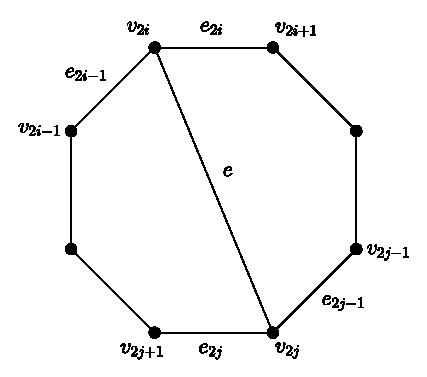
\includegraphics[width=.85\linewidth]{KernelMengerianO-fig1a}
  \caption{Case $1$}
  \label{fig1a}
\end{subfigure}%
\begin{subfigure}{.4\textwidth}
  \centering
  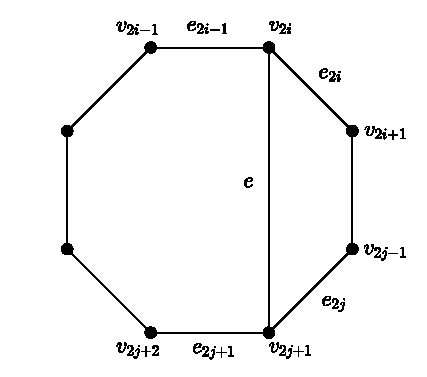
\includegraphics[width=.845\linewidth]{KernelMengerianO-fig1b}
  \caption{Case $2$}
  \label{fig1b}
\end{subfigure}
\caption{Chord $e \in C$}
\end{figure}

\begin{proof}[Proof of Lemma \ref{lem:prf3} \emph{(}i\emph{)}-\emph{(}iii\emph{)}]
The lemma holds trivially for edges in categories $(i)$ and $(iii)$, since edges in $(i)$ and $(iii)$ are dominated by consecutive edges from some $C\in E_{1/2}(x)$.

To prove the lemma holds for category $(ii)$, we distinguish two cases by the parity of endpoints of chord $e$ in $C$. We first show that $e$ cannot be a chord in any $C$ such that endpoints of $e$ have the same parity in $C$. Assume to the contrary that chord $e$ have the same parity in some $C\in E_{1/2}(x)$. Without loss of generality, let $e=v_{2i}v_{2j}$.

If $e_{2i}\prec e$, it follows that $e_{2i-1}\prec e$. Since $x(\varphi(e))=1$, $e\prec e_{2j-1}$ and $e\prec e_{2j}$ follow. However, $v_{2i} e v_{2j} e_{2j} v_{2j+1} \ldots v_{2i-1} e_{2i-1} v_{2i}$ form an odd cycle with cyclic preferences, a contradiction. Hence, $e\prec e_{2i}$.

Similarly, if $e_{2j}\prec e$, it follow that $e_{2j-1}\prec e$. Eqaulity $x(\varphi(e))=1$ implies that $e\prec e_{2i}$ and $e\prec e_{2i-1}$. However, $v_{2i} e_{2i} v_{2i+1} \ldots v_{2j-1} e_{2j-1} v_{2j} e v_{2i}$ form an odd cycle with cyclic preferences, a contradiction. Hence, $e\prec e_{2j}$. 

Now $e\prec e_{2i}$ and $e\prec e_{2j}$, it follows that $e_{2i-1}\prec e$ and $e_{2j-1}\prec e$ since $x(\varphi(e))=1$. But in this case the two odd cycles with cyclic preferences mentioned above occur at the same time. 

Therefore, $e$ cannot be a chord whose endpoints have the same parity in any $C$. It remains to show that in the latter case, dominating edges of chord $e$ have different parity. Without loss of generality, let $e=v_{2i} v_{2j+1}$.

If $e_{2i}\prec e$ or $e_{2j+1}\prec e$, it follows that $e_{2i-1}\prec e$ or $e_{2j}\prec e$ respectively. Then $e$ is dominated by two consecutive edges from $C$, which is trivial.  So assume that $e\prec e_{2i}$ and $e\prec e_{2j+1}$. Since $x(\varphi(e))=1$, it follows that $e_{2i+1}\prec e$ and $e_{2j}\prec e$. Therefore, e is dominated by two nonadjacent edges with different parity.
\end{proof}

To prove the remaining part of Lemma \ref{lem:prf3}, we need some preparations. Let $F_i$ be the set of hanging edges of $C_i\in E_{1/2}(x)$ in category $(iv)$ of Lemma \ref{lem:prf3}. Clearly, if $e\in F_i$, then there exists $F_j$ ($j\not= i$) such that $e\in F_j$. Analogous to the definition of cycles with cyclic preferences, we call $P=v_1 v_2 \ldots v_l$ a \textit{$v_1 v_l$-path with linear preferences} if $v_iv_{i+1}\prec_{v_{i+1}}v_{i+1}v_{i+2}$ for $i=1,2,\ldots,l-2$. We have the following characterization for any two vertices from the same component of the induced subgraph $\cup_{i=1}^{i=r} (F_i\cup C_i)$ of $\hat{H}$.

\begin{figure}
\centering
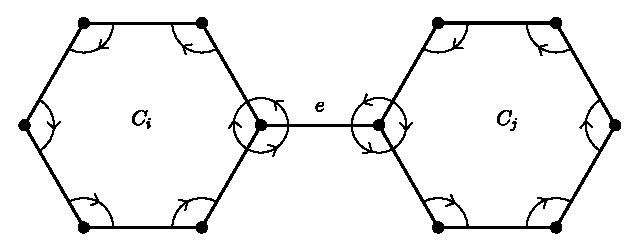
\includegraphics[scale=0.85]{KernelMengerianO-fig2}
\caption{$e\in F_i\cap F_j$}
\end{figure}

\begin{lemma}
\label{lem:prf4}
Given Lemma \ref{lem:prf3} is true, for any two vertices in the same component of induced subgraph $\cup_{i=1}^{i=r}(F_i\cup C_i)$, there exists a path with linear preferences between them. Moreover, if they have the same parity, the path is of even length; if they have different parity, the path is of odd length. 
\end{lemma}
\begin{proof}
When vertices are from the same cycle $C\in E_{1/2}(x)$, the lemma holds trivially. Hence take $v^s \in C_s$ and $v^t\in C_t$ where $s\not=t$. The existence of paths with linear preferences is trivial. Without loss of generality, consider a $v^s v^t$-path with linear preferences. We prove this lemma by induction on the number $\tau$ of cycles from $E_{1/2}(x)$ involved in the $v^s v^t$-path. Clearly, $\tau\geq 2$.

When $\tau=2$. Take $v^s_+ v^t_-\in F_s\cap F_t$. Let $P_s$ be the path with linear preferences from $v^s$ to $v^s_+$ in $C_s$ and $P_t$ be the path with linear preferences from $v^t_-$ to $v^t$ in $C_t$. Then $P=v^sP_s v^s_+ v^t_- P_t v^t$ is a $v^s v^t$-path with linear preference. By Lemma \ref{lem:prf3}, $v^s_+$ and $v^t_-$ have different parity since $v^s_+ v^t_-\in F_s\cap F_t$. If $v^s$ and $v^t$ have the same parity, then lengths of $P_s$ and $P_t$ have different parity, implying that $P$ is of even length; if $v^s$ and $v^t$ have different parities, then lengths of $P_s$ and $P_t$ have the same parity, implying that $P$ is of odd length.

Now assume that lemma is true for all $\tau\geq 2$. Let $C_{k_1},\ldots,C_{k_\tau},C_{k_{\tau+1}}$ be cycles from $E_{1/2}(x)$ involved along the $v^s v^t$-path with linear preferences. Take $v^{k_{\tau}}_+ v^{k_{\tau+1}}_- \in F_{k_{\tau}}\cap F_{k_{\tau+1}}$. Let $P_{s, k_{\tau}}$ denote the $v^s v^{k_{\tau}}_+$-path and $P_{k_{\tau},t}$ denote the $v^{k_{\tau}}_+ v^t$-path, both of which have linear preferences. Clearly, $P=v^sP_{s,k_\tau} v^{k_\tau}_+ P_{k_\tau, t} v^t$ is a $v^s v^t$-path with linear preferences. Since $P_{s, k_{\tau}}$ is a path involving only $\tau$ cycles and $P_{k_{\tau},t}$ is a path involving only two cycles, their lengths both depend on the parity of their endpoints. It is easy to see that $P$ is of even length when $v^s$ and $v^t$ have the same parity and $P$ is of odd length when $v^s$ and $v^t$ have different parity.
\end{proof}

\begin{proof}[Proof of Lemma \ref{lem:prf3} \emph{(}iv\emph{)}]
It suffices to prove that the lemma holds for each component in the induced subgraph $\cup_{i=1}^{i=r} F_i\cup C_i$. We apply induction on the number $\alpha$ of cycles from $E_{1/2}(x)$ in a component.

When $\alpha=1$, it is trivial.

Assume that Lemma \ref{lem:prf3} $(iv)$ is true for components with $\alpha\geq 1$ cycles from $E_{1/2}(x)$. We consider a component with $\alpha +1$ cycles $C_1, C_2, \ldots, C_{\alpha}, C_{\alpha+1}$ from $E_{1/2}(x)$. We further require that $C_{\alpha+1}$ is not a cut vertex if we view these cycles as vertices in this component.
Hence deleting $C_{\alpha+1}$ yields a new component with $\alpha$ cycles, and Lemma \ref{lem:prf3} applies to the resulting new component. It remains to show that edges in $F_{\alpha+1}$ satisfy Lemma \ref{lem:prf3}. If there exists edge $e\in F_{\alpha+1}$ violating Lemma \ref{lem:prf3}, we relabel vertices and edges in $C_{\alpha+1}$. We will show that after at most one relabeling, all edges in $F_{\alpha+1}$ satisfy Lemma \ref{lem:prf3}. We prove it by contradiction. Let $f_1,f_2 \in F_{\alpha +1}$ be edges such that $f_1$ satisfies Lemma \ref{lem:prf3} but $f_2$ violates Lemma \ref{lem:prf3}. For $i=1,2$, let $f_i=u_i w_i$, where $u_i$ is a vertex in the resulting new component and $w_i$ is a vertex in $C_{\alpha+1}$. By assumption, $u_1$ and $w_1$ have different parity and $u_2$ and $w_2$ have the same parity.

By Lemma \ref{lem:prf4}, there exists a path $P_\alpha$ with linear preferences between $u_1$ and $u_2$. Without loss of generality, let $P_\alpha$ be a $u_1 u_2$-path with linear preferences. There also exists a path $P_{\alpha+1}$ with linear preferences from $w_2$ to $w_1$. Now $u_1 P_\alpha u_2 f_2 w_2 P_{\alpha+1} w_1 f_1 u_1$ form a cycle $\hat{C}$ with cyclic preferences. We will show that $\hat{C}$ is an odd cycle with cyclic prefereces. 

If $u_1$ and $u_2$ have the same parity, then $w_1$ and $w_2$ have different parity. It follow that $P_\alpha$ is of even length and $P_{\alpha+1}$ is of odd length. Hence $\hat{C}$ is an odd cycle with cyclic preferences.

If $u_1$ and $u_2$ have different parity, then $w_1$ and $w_2$ have the same parity. It follows that $P_\alpha$  is of odd length and $P_{\alpha+1}$ is of even length. Hence $\hat{C}$ is an odd cycle with cyclic preferences again.

Either case leads to an odd cycle with cyclic preferences, a contradiction.
\end{proof}

\begin{proof}[Proof of Lemma \ref{lem:prf1}]
By Lemma \ref{lem:prf3}, each $1/2$-integral point $x\in FSM(\hat{H},\hat\prec)$ can be perturbed by $\epsilon z$ for small $\epsilon$ without leaving $FSM(\hat{H},\hat\prec)$. Hence $1/2$-integral points can not be vertices of $FSM(\hat{H},\hat\prec)$. By Theorem \ref{thm:AbelRoth94}, $SM(\hat{H},\hat\prec)=FSM(\hat{H},\hat\prec)$ follows. 
\end{proof}

\begin{proof}[Proof of Theorem \ref{thm:main}]
It suffices to show the equivalence among $(i)$, $(iii)$ and $(iv)$. Without loss of generality, assume that $D$ is an orientation of line multigraph $L(H)$ such that any two vertices in $H$ are joined by at most two edges and parallel edges in $L(H)$ are orientated oppositely. When $D$ is clique-acyclic, $D$ is associated with a preference system $(H,\prec)$. Hence $\sigma(D)$ can be viewed as a linear system defined on preference system $(H,\prec)$ and consisting of constraints (\ref{constraints:1})-(\ref{constraints:5}) where constraints (\ref{constraints:1}), (\ref{constraints:2}) and $(\ref{constraints:5})$ form the Rothblum system $\pi(H,\prec)$.

Assume $D$ is good. Then the preference system $(H,\prec)$ constructed from $D$ admits no odd cycle with cyclic preferences and so is $(\hat{H},\hat\prec)$, where $\hat{H}$ is a spanning subgraph of $H$ obtained by keeping one edge between every pair of adjacent vertices in $H$ and $\hat\prec$ is the restriction of $\prec$ on $\hat{H}$. By Lemma \ref{lem:prf1}, $FSM(\hat{H},\hat\prec)$ is integral. Integrality of $FSM(H,\prec)$ follows from Lemma \ref{lem:reduct6}. Hence constraints (\ref{constraints:3}) and (\ref{constraints:4}) are both redundant in $\sigma(D)$ which defines $FK(D)$. Therefore $FK(D)=FSM(H,\prec)$, implying that $FK(D)$ is integral. Similar arguments apply to any induced subgraphs of $D$. Hence $(i)\implies (iii)$. Further notice that, by Theorem \ref{thm:ChenDing12} integrality of $FSM(\hat{H},\hat\prec)$ implies total dual integrality of $\pi(\hat{H},\hat\prec)$. Then total dual integrality of $\pi(H,\prec)$ follows from Lemma \ref{lem:reduct3}. Since $\pi(H,\prec)$ is part of $\sigma(D)$ and the other constraints (\ref{constraints:3}), (\ref{constraints:4}) are redundant in $\sigma(D)$, total dual integrality of $\sigma(D)$ follows. Similar arguments apply to any induced subgraphs of $D$. Therefore, $(i)\implies (iv)$.

To see $(iii)\implies (i)$, we prove it by contradiction. Observe that strong kernel idealness of  $D$ implies the existence of kernels for any induced subgraphs of $D$. Let $D$ be a digraph such that D is strongly kernel ideal but not good. Then there exists either a clique containing directed cycles or a directed odd cycle without chords and pseudochords in $D$. We show that neither case is possible. If $D$ has a clique containing directed cycles, we consider the subgraph induced on this clique. There is no kernel for this induced subgraph, a contradiction. If $D$ contains a directed odd cycle without chords and pseudochords, we restrict ourselves to the subgraph induced on this directed odd cycle. There is no kernel for this induced subgraph either, a contradiction.

To see $(iv)\implies (i)$, notice that $(iv)\implies (iii)$ is a directly result from a theorem by Edmonds and Giles \cite{EdmoGile77}.  Hence $(iv)\implies (i)$ follows from $(iii)\implies (i)$.

\end{proof}


\bibliographystyle{plain}
\bibliography{KernelMengerianO}
\nocite{Schr86}

\end{document}
